%!TeX root = main.tex
%!encoding = UTF-8 Unicode

\section{Demonstration of Switching Event Resolved Frequency Domain Analysis}
In this section the switching event resolved frequency domain analysis is demonstrated, which provides a more detailed analysis of the noise contribution of the different switching events.
The methodology is explained in detail in Section~\ref{subsec:SpectralSeparation}.
The test results are for a first generation, Robert Bosch SiC MOSFET operated at $\mi{V}{DC} = \SI{800}{V}$, $\mi{I}{load} = \SI{60}{A} = \mi{I}{N,MOSFET}$, and $\mi{R}{G} = \SI{5.6}{\Omega}$, with a commutation-loop inductance of $\mi{L}{\sigma} = \SI{24}{nH}$ and an ambient temperature of $T = \SI{30}{\celsius}$.

Figure~\ref{fig:MR_Demo_SpekSep_TD} shows the time-domain measurement results of the demonstration of switching event resolved frequency domain analysis.
The two measured voltages of the active and passive switch are separated into the four artificial signals of the active-on, active-off, passive-on, and passive-off switching events.



\begin{figure}[ht]
	\centering
	\begin{subfigure}[t]{\textwidth}
		\centering
		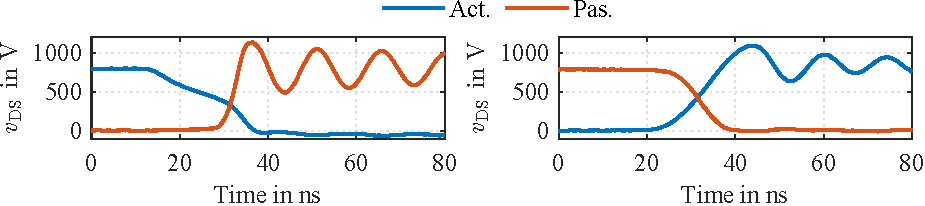
\includegraphics[scale = 1]{figures/6_Environment/MR_Demo_SpekSep/MR_Demo_SpekSep_ActPasVoltage_TD.pdf}
		\subcaption{Time-domain voltage measurement results of the active and passive switches.}
		\label{fig:MR_L_constE_Sweep_Voltage_TD}
	\end{subfigure} 
    
	\vspace{0.5cm}	
	
	\begin{subfigure}[t]{\textwidth}
		\centering
		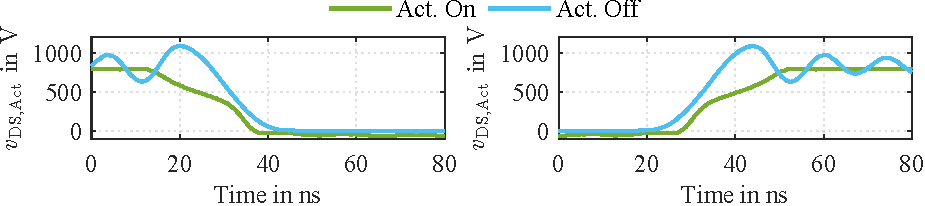
\includegraphics[scale = 1]{figures/6_Environment/MR_Demo_SpekSep/MR_Demo_SpekSep_ActVoltage_TD.pdf}
		\subcaption{Separated, artificial switching events of the active switch.}
		\label{fig:MR_L_constE_Sweep_ActVoltage_TD}
	\end{subfigure} 

	\vspace{0.5cm}

	\begin{subfigure}[t]{\textwidth}
		\centering
		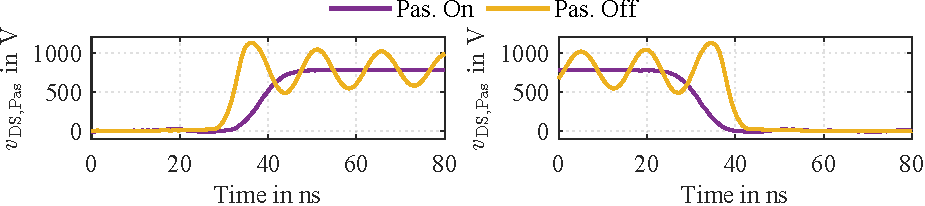
\includegraphics[scale = 1]{figures/6_Environment/MR_Demo_SpekSep/MR_Demo_SpekSep_PasVoltage_TD.pdf}
		\subcaption{Separated, artificial switching events of the passive switch.}
		\label{fig:MR_L_constE_Sweep_PasVoltage_TD}
	\end{subfigure} 

	\caption{Time-domain results of the demonstration of switching event resolved frequency domain analysis.}
	\label{fig:MR_Demo_SpekSep_TD}
\end{figure}


These measurements show the typical behavior of a MOSFET switched with a constant gate resistance at room temperature. 
The observations can be summarized as follows:
\begin{enumerate}
	\item The passive-off event exhibits a higher overvoltage than the active-off event (\SI{1130}{V} compared with \SI{1080}{V}), and this overvoltage increases with temperature because the body diode stores more bipolar charge.
	\item The passive-off event responds purely passively to the excitation transient, whereas the active-off event initially shows an approximately linear voltage increase controlled by the gate driver. This is followed by an inductive overshoot, only after which the output capacitance and the commutation-cell inductance begin to oscillate passively.
	\item The on-events also behave differently: the active-on event initially exhibits a voltage drop caused by the inductive voltage drop across the commutation-cell inductance, followed by the actual voltage commutation controlled by the gate driver. This creates two distinct transient times, and the faster or larger one dominates the spectrum.
	\item In contrast, the passive-on event shows a smooth voltage transient, which is the reaction of the passive $LC$ tank to the controlled active-off transient and is therefore smoothed by the impedance of the tank.
\end{enumerate}

These time-domain observations provide the physical basis for the event-resolved interpretation of the frequency-domain spectra. To understand the impact of the four distinct switching events on the measured spectrum, the same snap-and-mirror method is applied to the corresponding high-pass measurements and combined with the TDF filter in post-processing. The resulting frequency-domain results are shown in \fref{fig:MR_Demo_SpekSep_FD}.
The general functionality of the snap-and-mirror method is demonstrated by the observation that, for both the active and passive switch emission spectra, one of the two contributing switching events (on or off) dominates specific frequency ranges, while the other contributes only marginally.

\begin{figure}[!t]
	\centering
	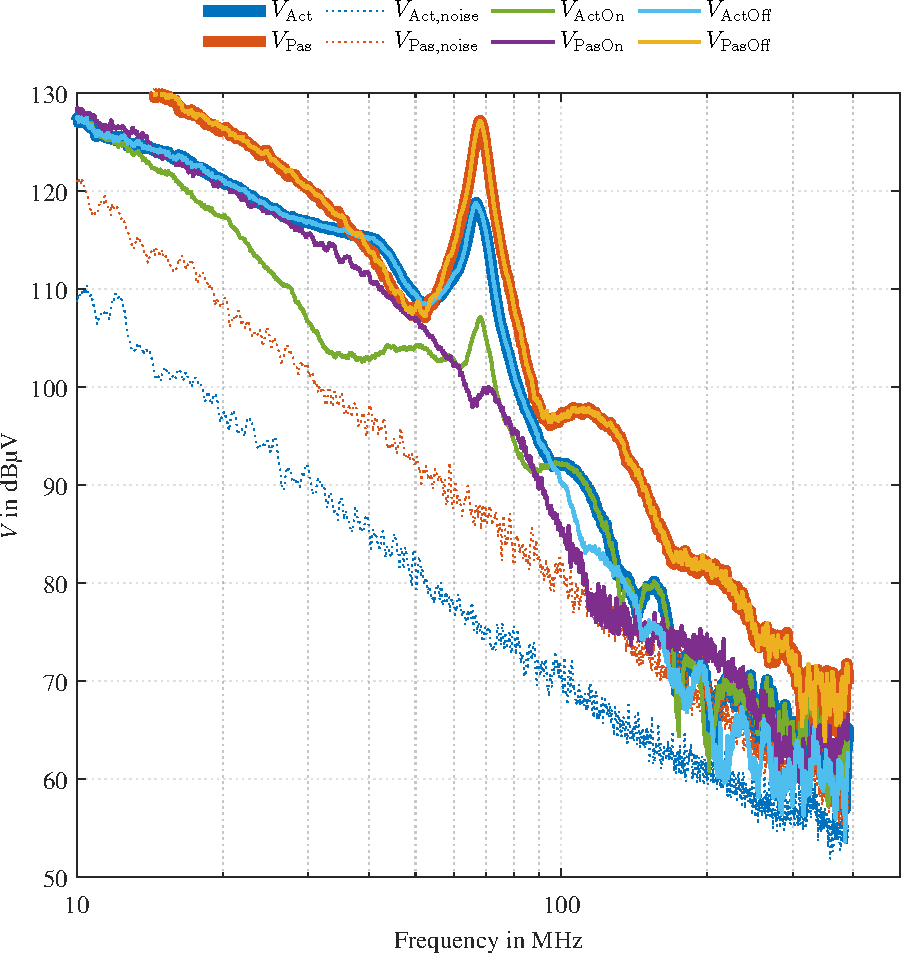
\includegraphics[scale = 1]{figures/6_Environment/MR_Demo_SpekSep/MR_Demo_SpekSep_FD.pdf}
	\caption{Frequency-domain measurement results of the demonstration of switching event resolved frequency domain analysis.}\label{fig:MR_Demo_SpekSep_FD}
\end{figure}

In addition, several consistent trends can be identified in the frequency-domain results over a wide range of operating conditions. These are summarized as follows:
\begin{enumerate}
	\item The passive switch, and in particular the passive-off event, exhibits consistently higher emission than the active switch. This trend is consistent with the general EMC experience in the laboratory and is attributed to the larger overvoltage and stronger ringing of the passive switch.
	\item For the active switch, the turn-off event dominates the lower-frequency range and the resonance region; however, above approximately \SI{100}{MHz}, the turn-on event becomes dominant and reaches up to \SI{8}{dB} higher emission. The exact crossover frequency depends on the switching speed.
	\item A slight mismatch between the resonance frequencies of the active and passive switch is observed (\SI{66}{MHz} compared with \SI{69}{MHz}). 
	This difference increases for smaller chip sizes and lower capacitances, as predicted by the coupling model in \cite{liu_modeling_2016}. 
	The underlying cause is the different coupling of the oscillation into the gate loop of the active switch and the passive switch, respectively.
	\item A small resonance is observed in the active-on event, which is attributed to imperfect shielding and capacitive coupling from the passive-off event into the active-on contribution. 
	This effect is not observed in the passive-on event because the active-off event is significantly smaller in amplitude and therefore couples less strongly.
	\item Although the passive-on transient is faster than the active-on transient, its emission is lower in the high-frequency range. 
	This is due to the second, faster transient of the active-on event, which is steeper than the initial inductive voltage drop and therefore contributes more strongly to the high-frequency spectrum.
	\item The noise floor of the passive switch is higher than that of the active switch. 
	This is a consequence of the larger signal amplitude and the associated requirement for a larger vertical scale on the oscilloscope, which increases the measurement noise floor.
\end{enumerate}

Overall, the event-resolved analysis provides a detailed and physically transparent decomposition of the total noise emission into its dominant switching-event contributors. 
This new method enables a much more precise assessment of the individual mechanisms that shape the measured spectrum and reveals which transient events actually limit the EMC performance at a given frequency range. In practical terms, this allows for targeted EMC debugging, since only the noisiest contributor determines the emission limit in a given frequency band. 
As a result, optimization can be focused on the dominant source rather than on the total waveform, enabling faster or more aggressive switching of other contributors without increasing the total emitted noise. 
This is particularly valuable for balancing switching losses and EMC performance, because the design space can be explored more deliberately when the limiting mechanism is known and not obscured by the aggregate signal.

